\chapter{Programación en RMI}

\section{Ejemplos}

Esta práctica contiene tres ejemplos que debemos ejecutar antes de proceder a escribir el ejercicio.
Los pasos de ejecución de todos los ejemplos son los siguientes.

\begin{itemize}
	\item
		Situarse en el directorio \texttt{src}, donde se encuentran todos los directorios de los paquetes de cada programa.
	\item
		Compilar con \texttt{javac} todos los ficheros \texttt{.java} del paquete deseado.
	\item
		Ejecutar \texttt{rmiregistry} desde el directorio \texttt{src}.
		Dado que esta orden es bloqueante, podemos utilizar el operador de paralelismo \texttt{\&}.
	\item
		Seguir las instrucciones de ejecución propias de cada fichero.
\end{itemize}

Por ejemplo, para compilar los ficheros del primer ejemplo, podemos ejecutar la siguiente orden:

\begin{lstlisting}[language=sh]
javac ejemplo1/*.java && rmiregistry
\end{lstlisting}

Presentamos los ejemplos a continuación:

\subsection{Envío de mensaje simple}

\begin{figure}[!ht]
\begin{center}
	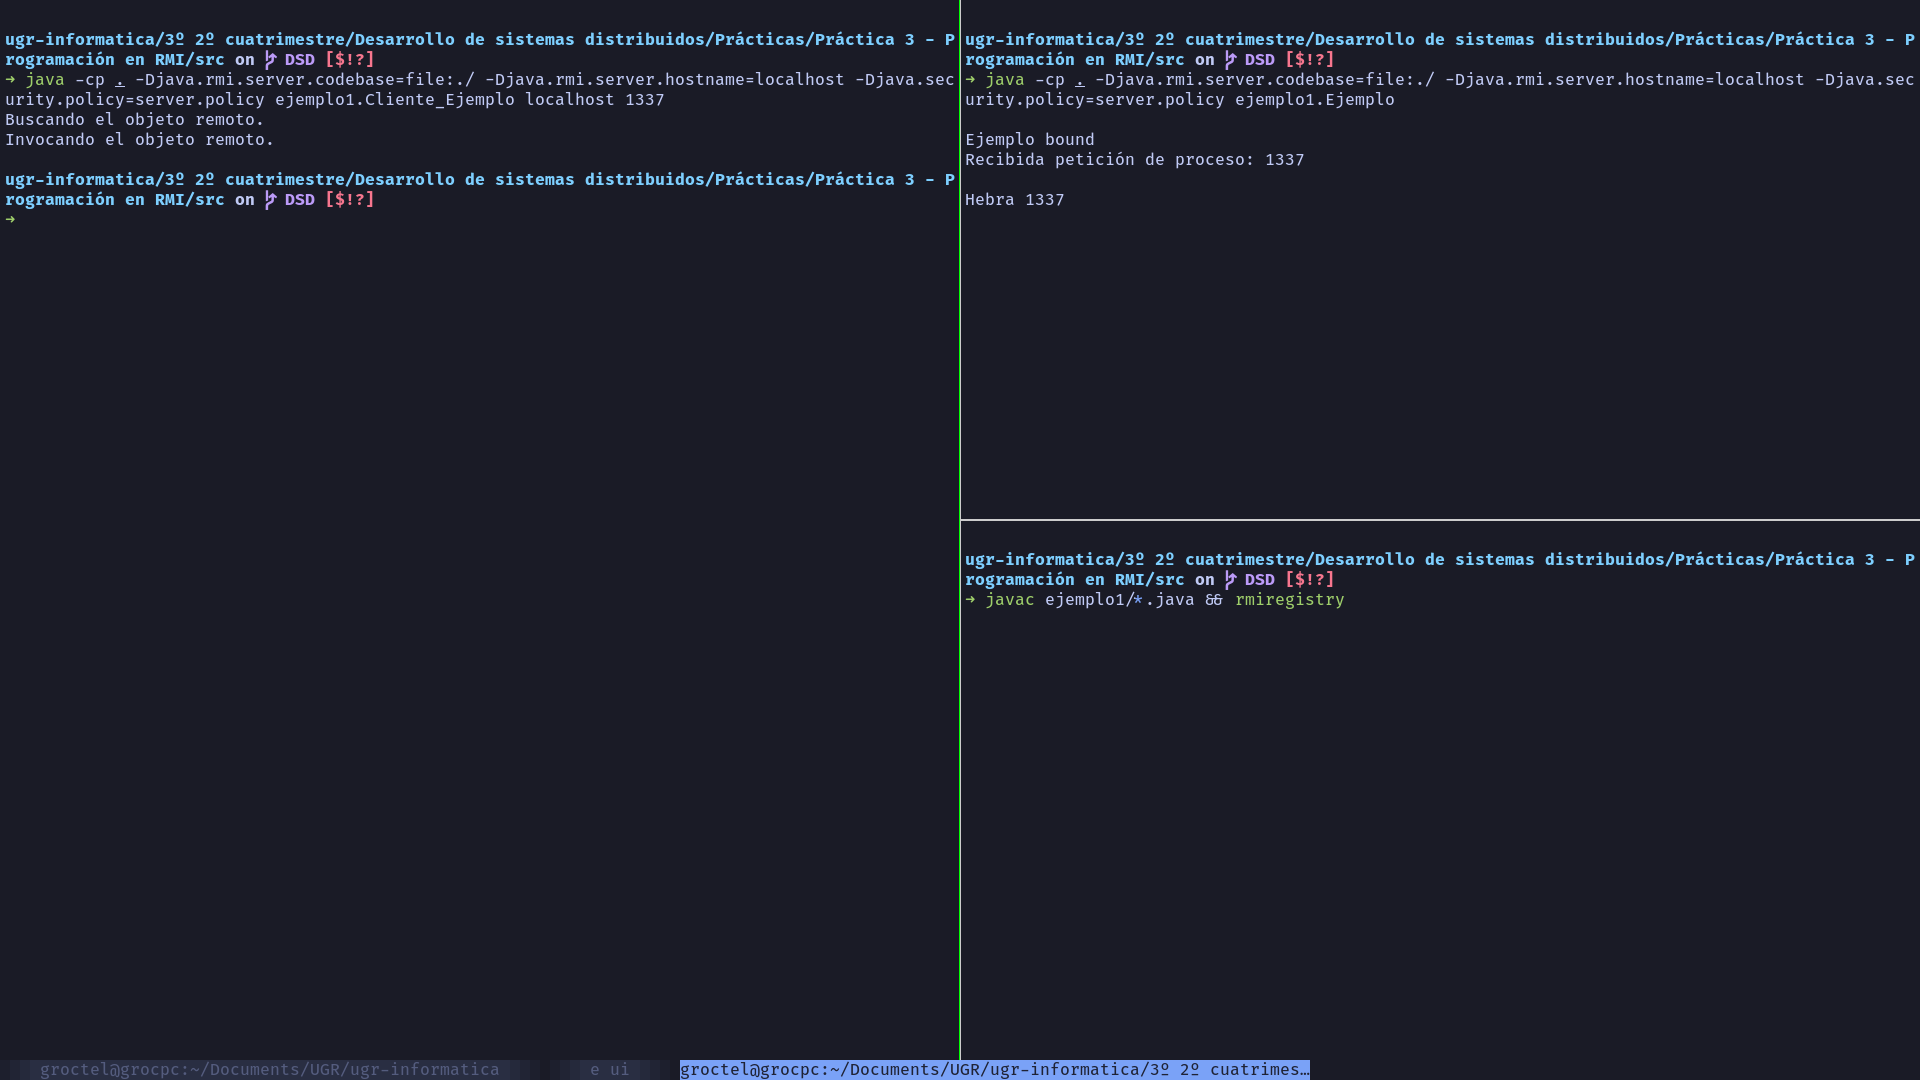
\includegraphics[scale=0.3]{rmi_ejemplo1}
\end{center}
\caption{Ejecución del primer ejemplo.}
\end{figure}

\pagebreak

Ejecutamos el servidor y el cliente con las siguientes órdenes:

\begin{lstlisting}[language=sh]
java -cp . -Djava.rmi.server.codebase=file:./ -Djava.rmi.server.hostname=localhost      -Djava.security.policy=server.policy ejemplo1.Ejemplo
java -cp . -Djava.rmi.server.codebase=file:./ -Djava.rmi.server.hostname=localhost      -Djava.security.policy=server.policy ejemplo1.Cliente_Ejemplo localhost 1337
\end{lstlisting}

Este programa es muy sencillo.
El servidor \texttt{Ejemplo} se configura con un nombre para que el cliente pueda buscarlo en el registro.
Cuando el cliente lo busca, crea un objeto local \texttt{Ejemplo\_I} para poder hacer una llamada a \texttt{Ejemplo}, que lo recibe e imprime el número de hebra.

\subsection{Envío de mensaje multihebrado}

\begin{figure}[!ht]
\begin{center}
	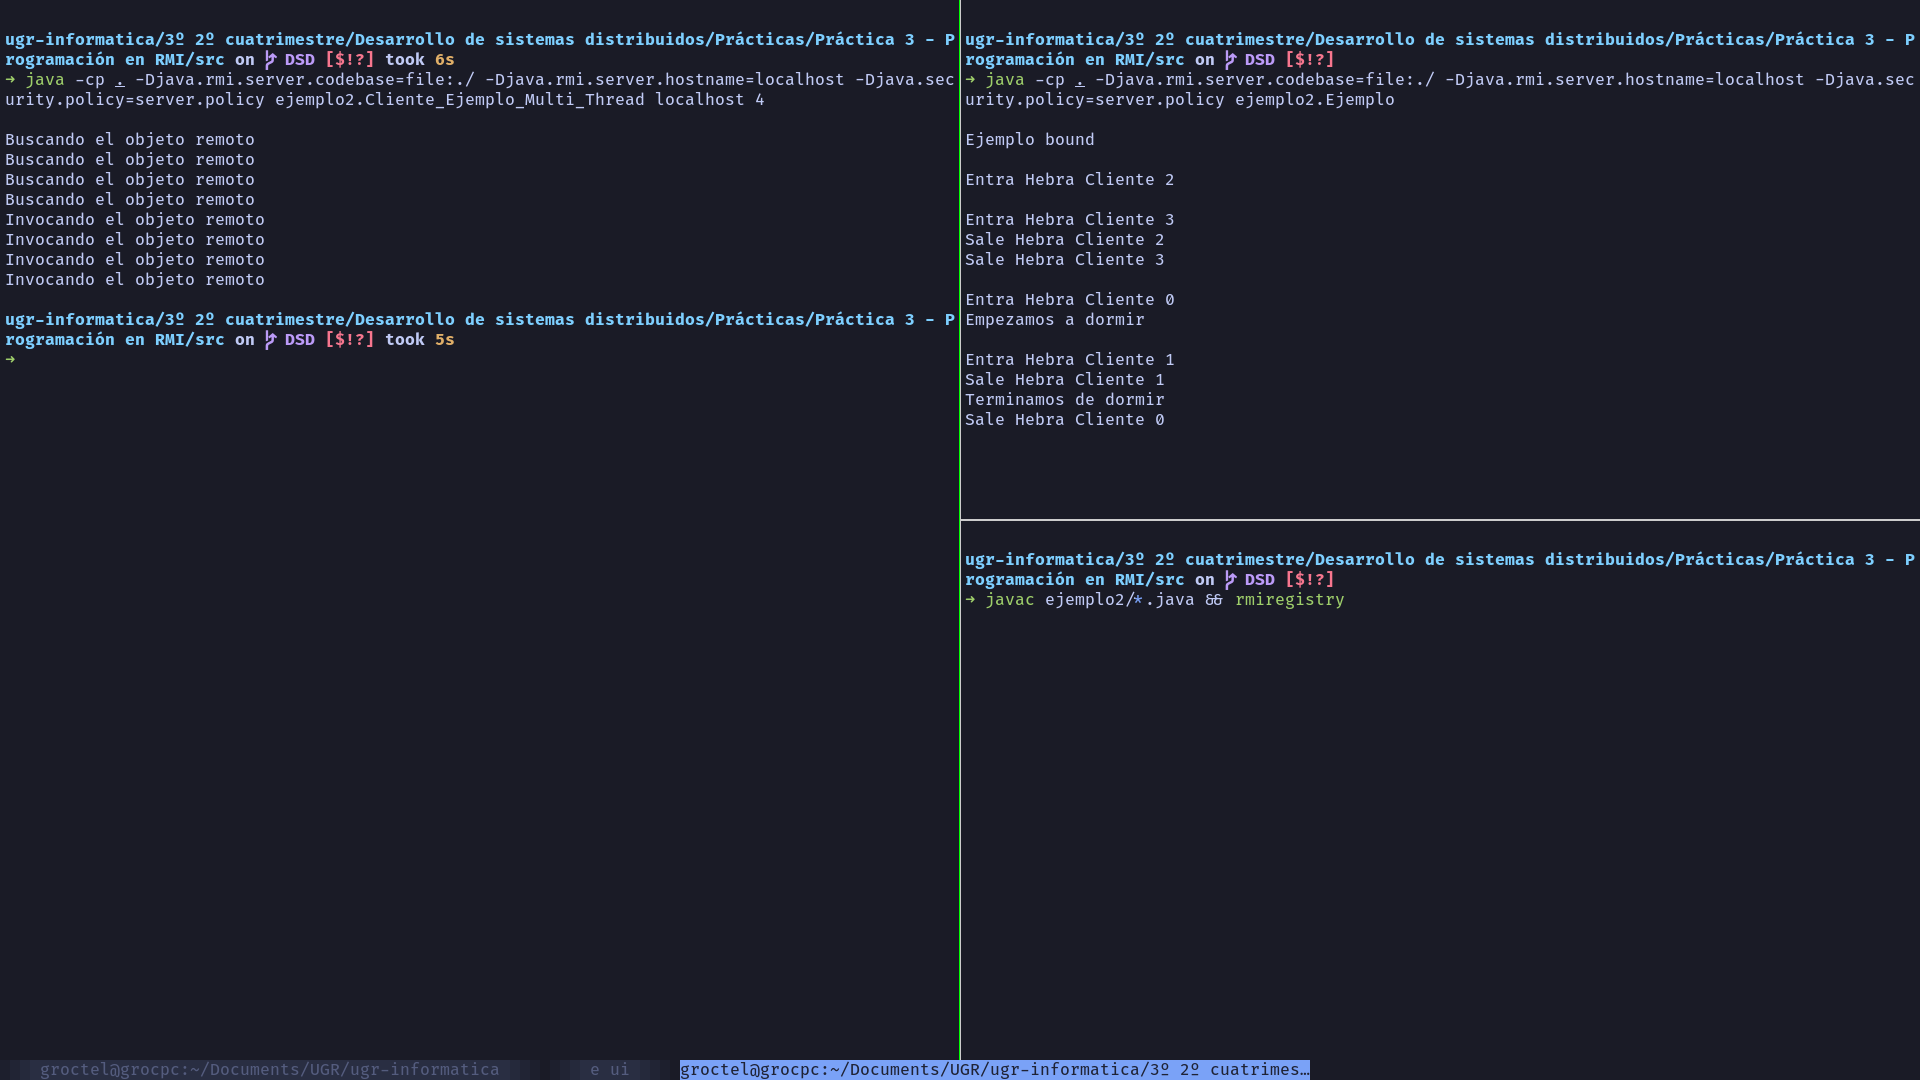
\includegraphics[scale=0.3]{rmi_ejemplo2}
\end{center}
\caption{Ejecución del segundo ejemplo.}
\end{figure}

Ejecutamos el servidor y el cliente con las siguientes órdenes:

\begin{lstlisting}[language=sh]
java -cp . -Djava.rmi.server.codebase=file:./ -Djava.rmi.server.hostname=localhost      -Djava.security.policy=server.policy ejemplo2.Ejemplo
java -cp . -Djava.rmi.server.codebase=file:./ -Djava.rmi.server.hostname=localhost      -Djava.security.policy=server.policy ejemplo2.Cliente_Ejemplo_Multi_Thread       localhost 10
\end{lstlisting}

Este ejemplo es similar al anterior, pero con la particularidad de que el servidor recibe las peticiones de las distintas hebras creadas por el cliente.

\pagebreak

\subsection{Contador}

\begin{figure}[!ht]
\begin{center}
	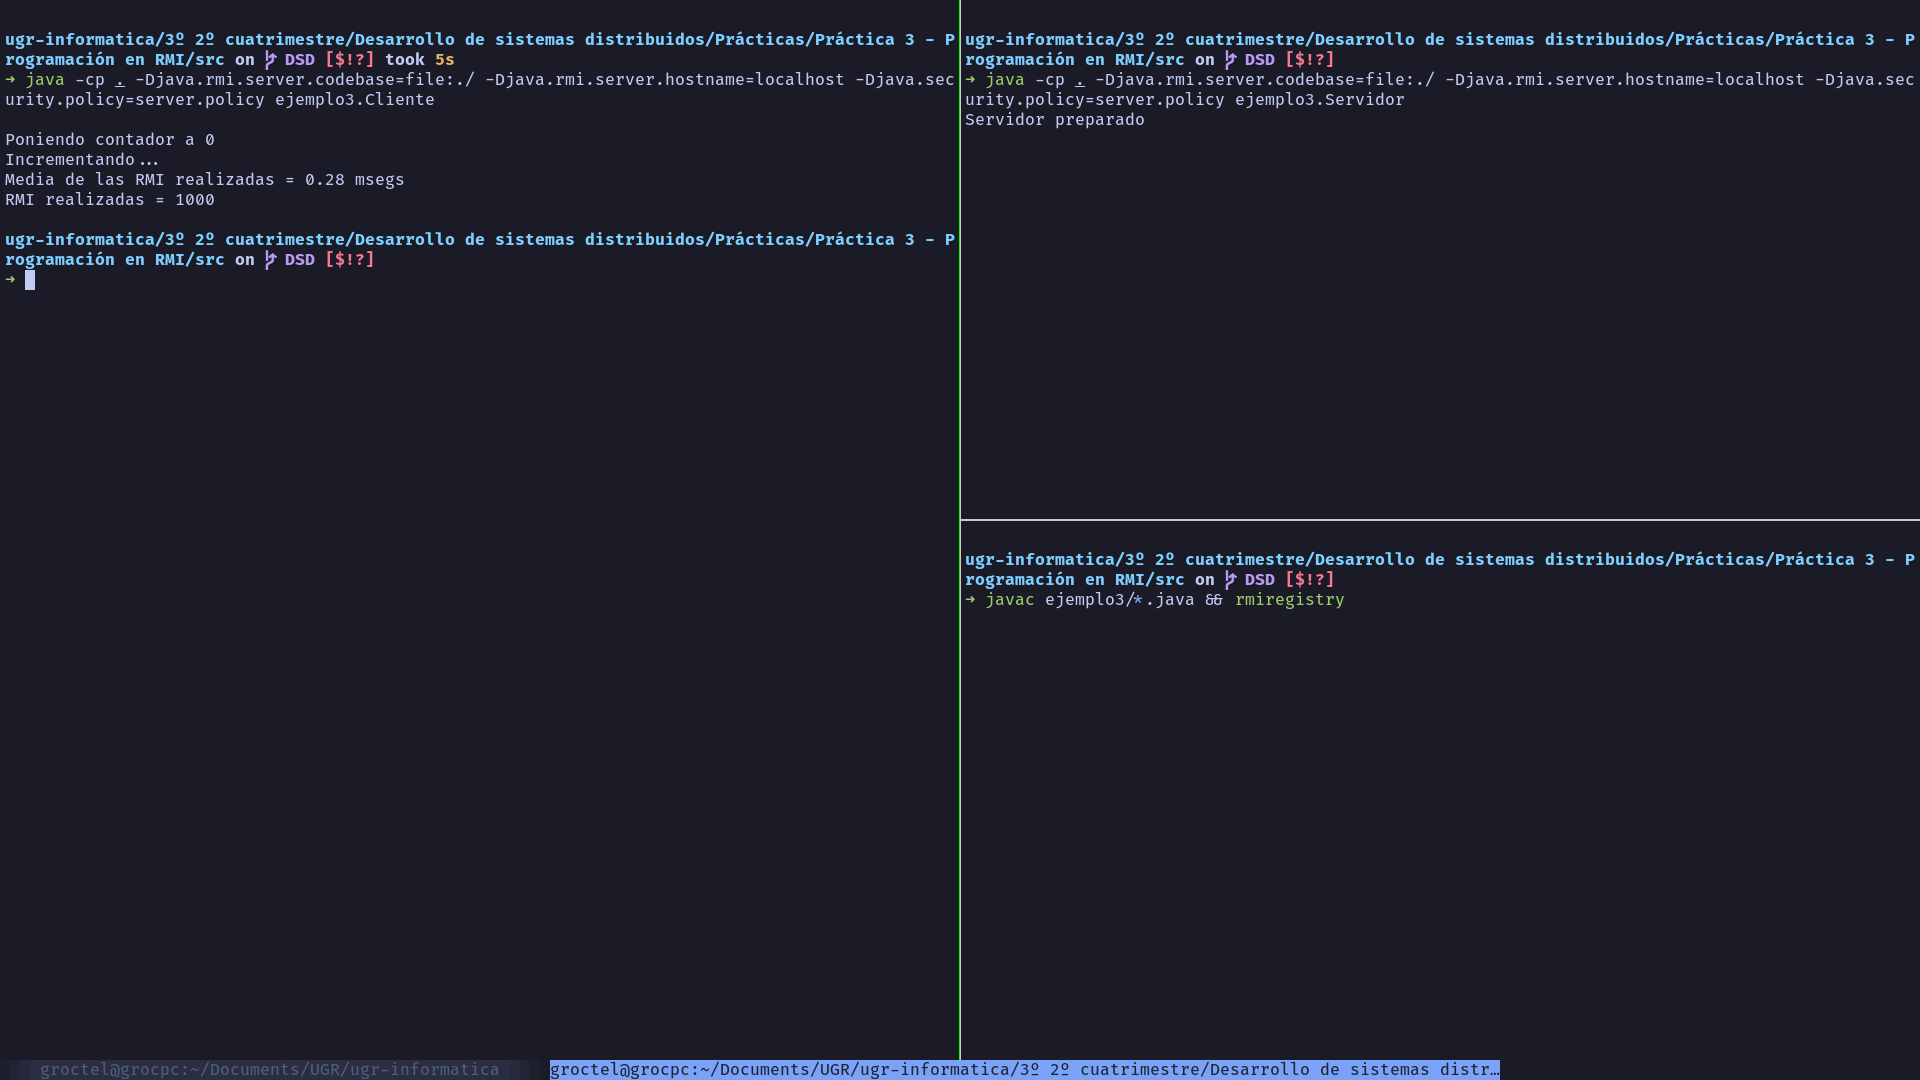
\includegraphics[scale=0.3]{rmi_ejemplo3}
\end{center}
\caption{Ejecución del tercer ejemplo.}
\end{figure}

Ejecutamos el servidor y el cliente con las siguientes órdenes:

\begin{lstlisting}[language=sh]
java -cp . -Djava.rmi.server.codebase=file:./ -Djava.rmi.server.hostname=localhost      -Djava.security.policy=server.policy ejemplo3.Servidor
java -cp . -Djava.rmi.server.codebase=file:./ -Djava.rmi.server.hostname=localhost      -Djava.security.policy=server.policy ejemplo3.Cliente
\end{lstlisting}

El cliente de este ejemplo realiza varias llamadas a un objeto remoto \texttt{Contador} para incrementar un valor local y devuelve el tiempo que ha tardado en hacer el número de peticiones indicado en el código.

\section{Ejercicio}

\begin{figure}[!ht]
\begin{center}
	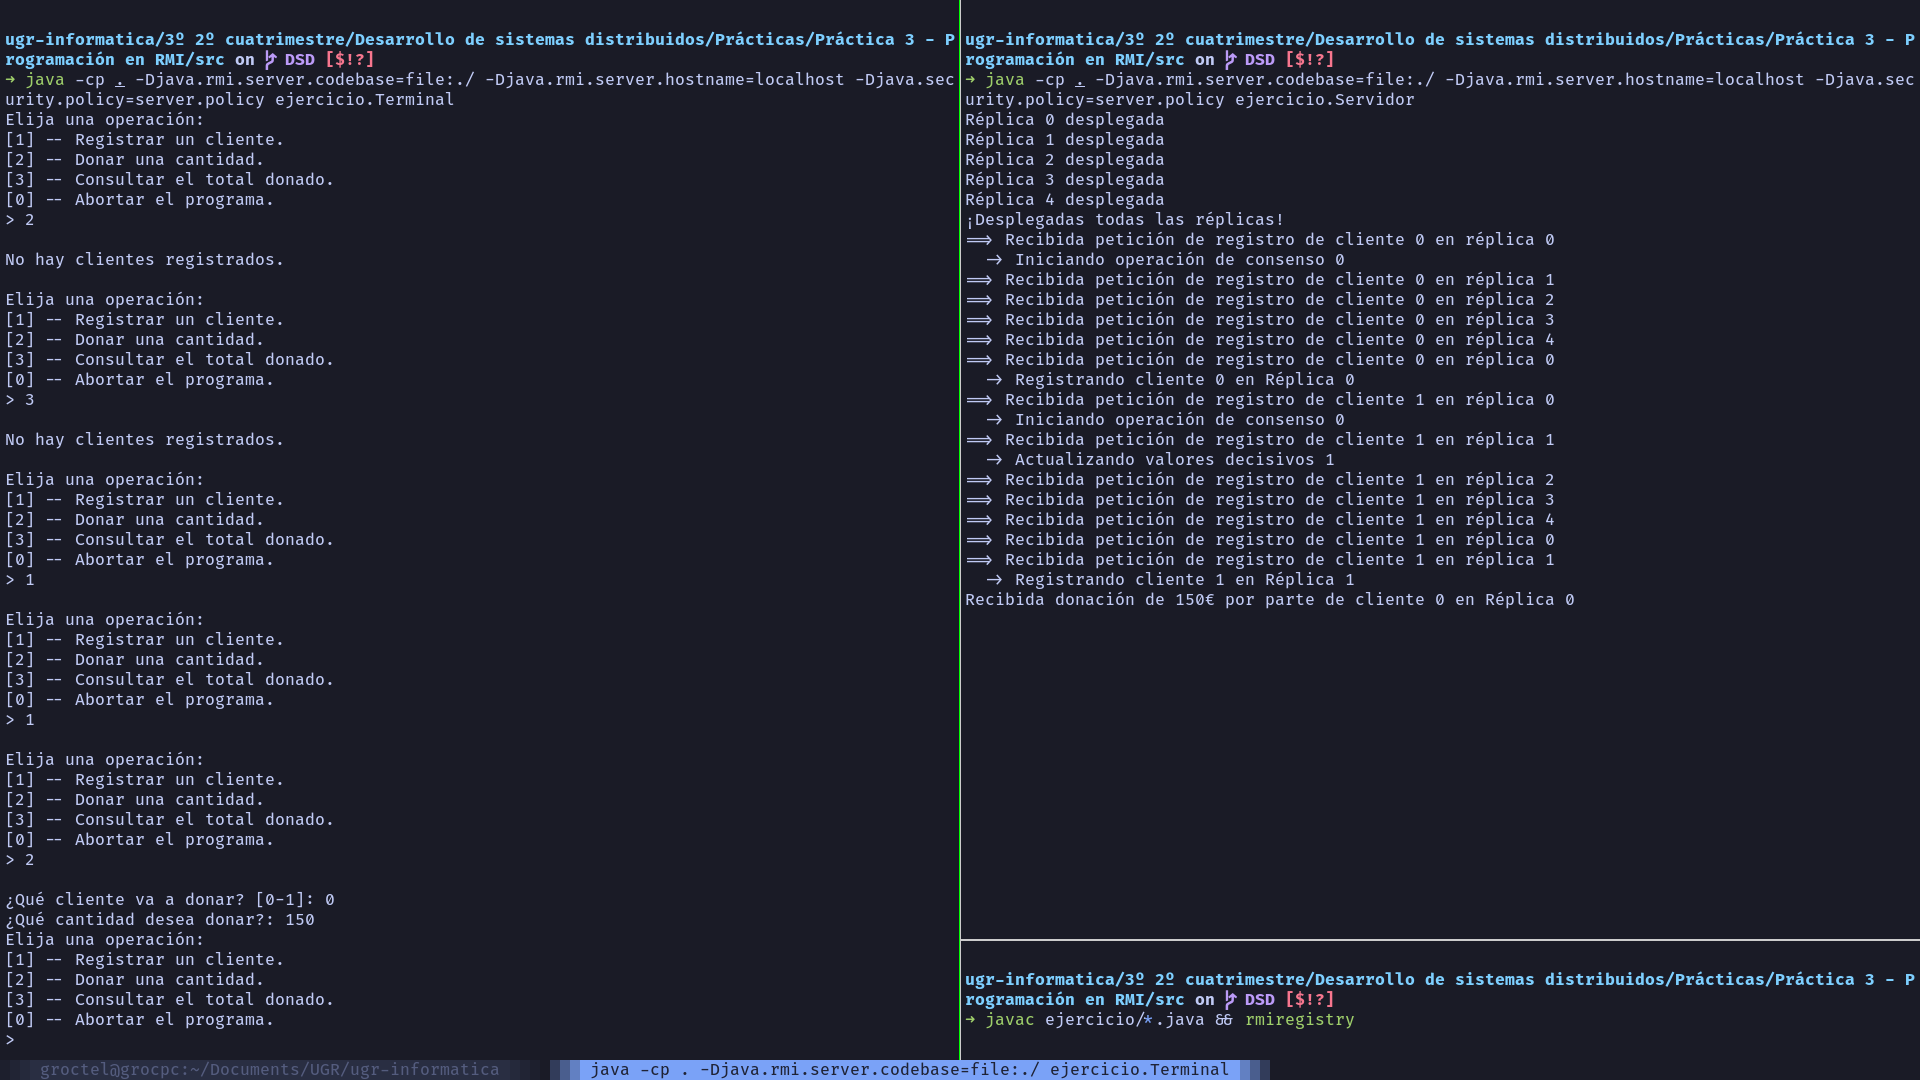
\includegraphics[scale=0.3]{rmi_ejercicio_1}

	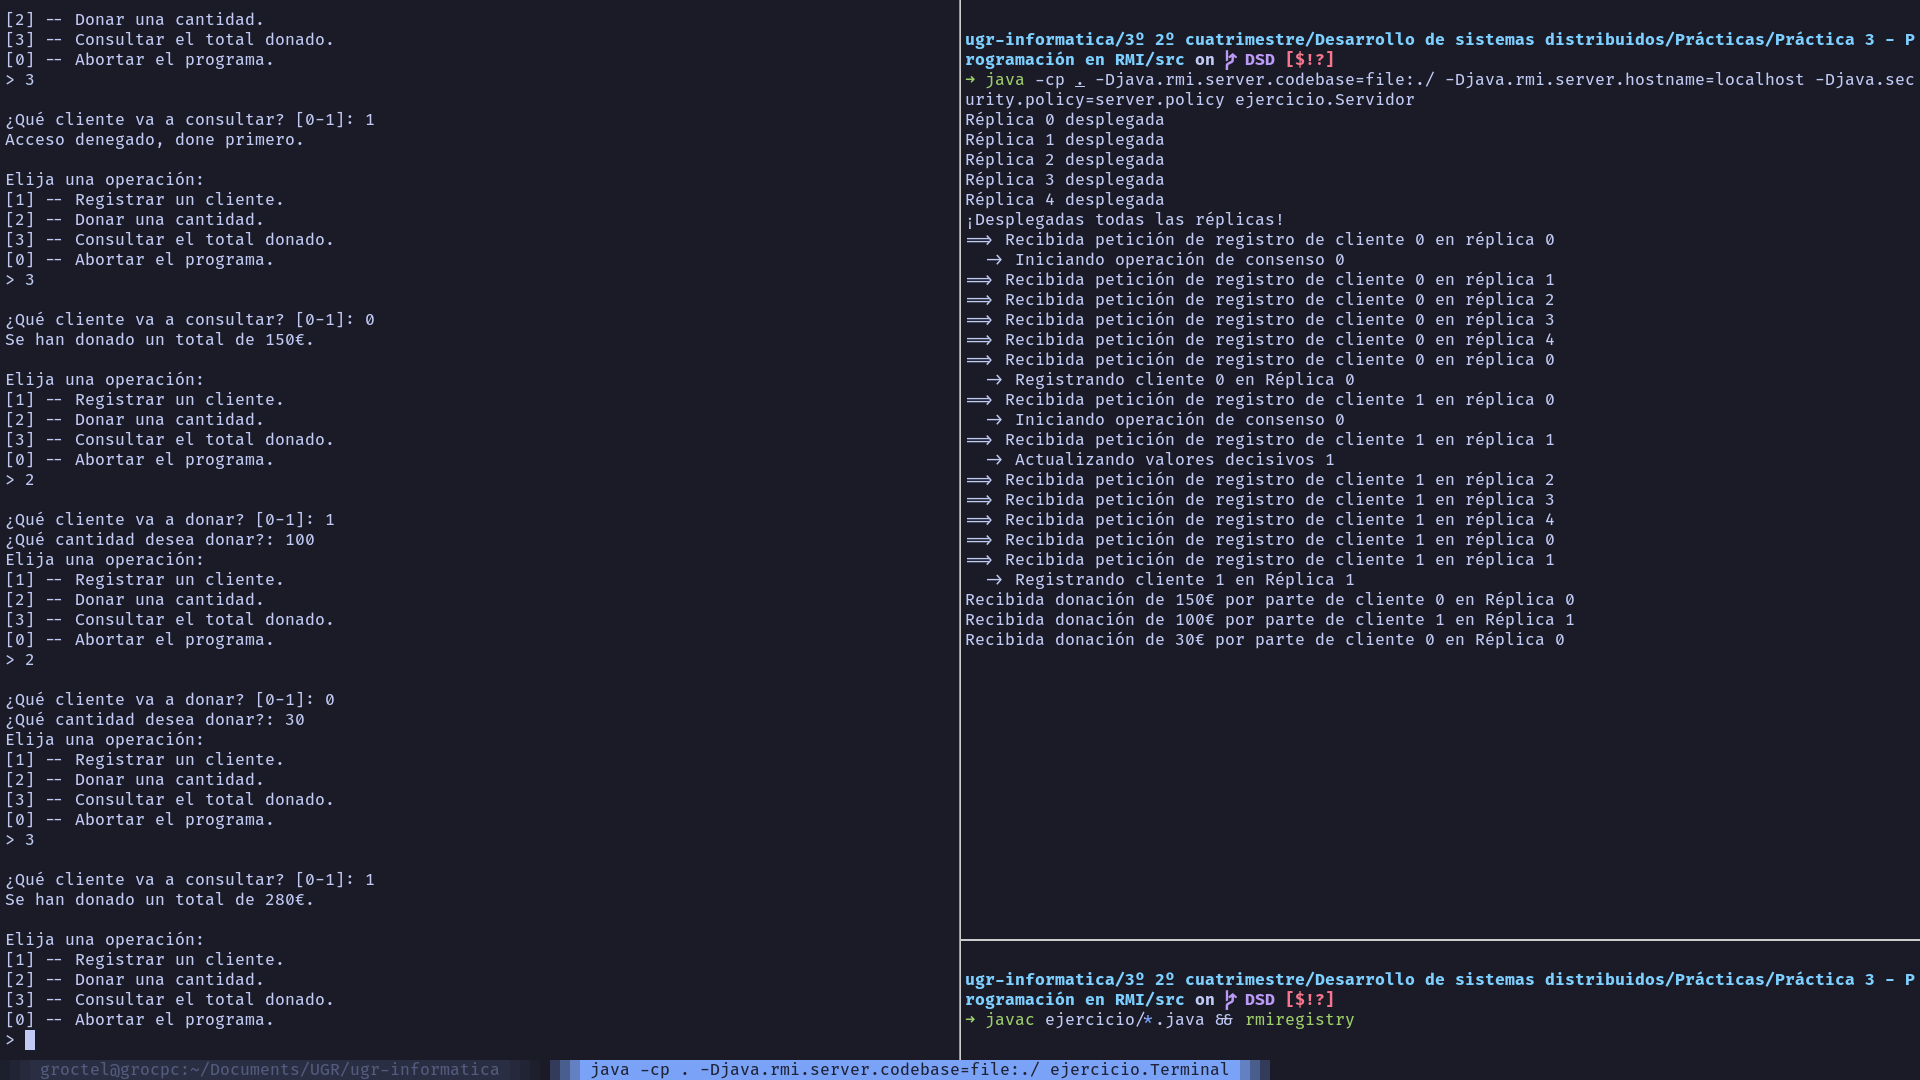
\includegraphics[scale=0.3]{rmi_ejercicio_2}
\end{center}
\caption{Ejecución del tercer ejemplo.}
\end{figure}

Ejecutamos el servidor y el cliente con las siguientes órdenes:

\begin{lstlisting}[language=sh]
java -cp . -Djava.rmi.server.codebase=file:./ -Djava.rmi.server.hostname=localhost      -Djava.security.policy=server.policy ejercicio.Servidor
java -cp . -Djava.rmi.server.codebase=file:./ -Djava.rmi.server.hostname=localhost      -Djava.security.policy=server.policy ejercicio.Terminal
\end{lstlisting}

En este ejercicio hemos creado una clase \texttt{Cliente} que almacena los datos del cliente, una clase \texttt{Réplica} que almacena la instancia de cada una de las réplicas que conforman la estructura del servidor y se crean mediante una clase auxiliar \texttt{Servidor} y una clase \texttt{Terminal} que crea la interfaz de usuario a la que accede el cliente.

Las réplicas se comunican entre sí en forma de anillo, de forma que todas conocen el número de réplicas totales y se comunican con la siguiente.
A la hora de registrar un cliente, se van intercambiando el objeto hasta decidir quién de ellas es la que lo aloja (la que menor \texttt{id} tenga de todas las réplicas con el menor número de registrados).
Para tomar las decisiones, las réplicas comparten la réplica candidata a ser la que registre al usuario (\texttt{replica\_decisiva}), su total de registrados (\texttt{valor\_decisivo}) y una bandera que indica si se ha tomado la decisión  (\texttt{decision\_ejecutada}).
Este diseño se ha hecho porque es mucho más eficiente que todos los objetos de la misma clase compartan datos miembro estáticos que pasarlos como argumento constantemente.

La gestión de las donaciones dentro de las réplicas se ha hecho en un \texttt{HashMap}, que es lo más sencillo y permite evaluar fácilmente el subtotal de una réplica creando una colección de sus valores e iterando por ella.

Para gestionar la consulta del total donado por clientes que no hayan donado, las réplicas devuelven un valor nulo (en este caso \texttt{0}, que es imposible que se dé ya que se requiere al menos una donación para la consulta).
